\documentclass[12pt,twoside]{article}
\usepackage{jmlda}
\newcommand{\hdir}{.}
\usepackage{hyperref}       % clickable links
\usepackage{lineno}
\usepackage{graphicx,multicol}
\usepackage{cite}
\usepackage{tikz}
\usetikzlibrary{shapes,arrows,shadows}
\newtheorem{theorem}{Теорема}
\newtheorem{statement}{Утверждение}
\usepackage{pb-diagram}
\usepackage{tikz-cd}


\bibliographystyle{jmlda_eng}
%\renewcommand{\baselinestretch}{1.4}


\newcommand{\bx}{\mathbf{x}}
\newcommand{\by}{\mathbf{y}}
\newcommand{\bw}{\mathbf{w}}
\newcommand{\bY}{\mathbf{Y}}
\newcommand{\bX}{\mathbf{X}}
\newcommand{\bu}{\mathbf{u}}
\newcommand{\bt}{\mathbf{t}}
\newcommand{\bp}{\mathbf{p}}
\newcommand{\bq}{\mathbf{q}}
\newcommand{\bg}{\mathbf{g}}
\newcommand{\bh}{\mathbf{h}}
\newcommand{\bv}{\mathbf{v}}
\newcommand{\be}{\mathbf{e}}
\newcommand{\bc}{\mathbf{c}}
\newcommand{\bP}{\mathbf{P}}
\newcommand{\bT}{\mathbf{T}}
\newcommand{\bQ}{\mathbf{Q}}
\newcommand{\bC}{\mathbf{C}}
\newcommand{\bE}{\mathbf{E}}
\newcommand{\bF}{\mathbf{F}}
\newcommand{\bU}{\mathbf{U}}
\newcommand{\bW}{\mathbf{W}}
\newcommand{\bD}{\mathbf{D}}
\newcommand{\bI}{\mathbf{I}}
\newcommand{\bJ}{\mathbf{J}}
\newcommand{\bB}{\mathbf{B}}
\newcommand{\btheta}{\boldsymbol{\theta}}
\newcommand{\bTheta}{\boldsymbol{\Theta}}



\title
	{Нелинейное снижение размерности в задачах декодирования временных рядов и прогнозирования}
\author
	{Мария Владимирова, Роман Исаченко}
\email
    {\href{mailto:vladimirova.maria@phystech.edu}{vladimirova.maria@phystech.edu}, 
    \href{mailto:isa-ro@yandex.ru}{isa-ro@yandex.ru}}
\organization
    {Московский физико-технический институт}
\abstract
	{В работе решается задача обнаружения зависимостей в прогнозируемой переменной. 
    Используется набор гомогенных моделей, восстанавливающих прогноз по общему для всех переменных описанию объектов. 
    Рассматривается линейная модель метода частный наименьших квадратов и ее предложенная нелинейная модификация. 
    Находятся оптимальные параметрические преобразования исходных пространств объектов и ответов. 
    Проводится вычислительный эксперимент на реальных данных объемов потребления электроэнергии и данных сигналов кортикограмм.

    \bigskip
	\noindent
	\textbf{Ключевые слова}: \emph {прогнозирование временных рядов; мультиколлинеарность; метод частных наименьших квадратов; PLS; нелинейный PLS} 
	}

\thanks{Проект поддержан грантом РФФИ \No 16-07-01155.}

\tikzcdset{
	arrow style=tikz,
	diagrams={>={Straight Barb[scale=0.8]}}}

\begin{document}
\maketitle


\linenumbers
%%%%%%%%%%%%%%%%%%%%%%%%%%%%%%%%%%%%%%%%%%%%%%%%%%%%%%%%%%%%%%%%%%%%%%%%%%%%%%
\section{1. Введение}
%%%%%%%%%%%%%%%%%%%%%%%%%%%%%%%%%%%%%%%%%%%%%%%%%%%%%%%%%%%%%%%%%%%%%%%%%%%%%%

В работе рассматривается задача прогнозирования временных рядов в случае наличия мультиколлинеарности в данных. Методы решения данной задачи сравниваются на двух наборах данных, имеющих избыточную информацию. 

Первый набор данных представляет собой временные ряды объема потребления электроэнергии в Варшаве. 
% Также в работе рассматривается задача прогнозирования потребления электроэнегрии на основе исторических данных. 
Электрическая энергия является важной движущей силой экономического развития, а точность прогнозов спроса является важным фактором, который ведет к успешному эффективному планированию. 
По этой причине энергетическим аналитикам необходимо руководство для лучшего выбора наиболее подходящих методов прогнозирования, чтобы обеспечить точные прогнозы тенденций потребления электроэнергии.
Предполагается, что значение сигнала в данный момент времени линейно зависит от предыдущих значений этого же сигнала, поэтому данные являются мультиколлинеарными.  


Второй набор данных взят из проекта Project Tycho, в котором изучалась проблема проектирования нейро-компьютерного интерфейса (BCI) для обмена информацией между мозгом и электронным устройством. Решается задача выбора функций в моделях регрессии в приложении к декодированию движения на основе электрокардиограмм (ECoG). 
Проблема состоит в том, чтобы предсказать траектории руки из временных рядов напряжения кортикальной активности. Описание функции каждой точки находится в пространственно-временной частотной области включает в себя сами временные ряды напряжения и их спектральные характеристики. Выбор функции имеет решающее значение для адекватного решения проблемы регрессии, поскольку электрокортикальные данные являются высокомерными и измерения коррелируют как во временной, так и в пространственной областях.

Система BCI улучшает умственные и физические возможности пользователя, обеспечивая прямую связь между мозгом и компьютером. BCI направлены на восстановление поврежденных функциональных возможностей пациентов с механическими или когнитивными нарушениями. В данной статье предлагается новый метод выбора признаков в прогнозировании движения и его реконструкции.
% Анализ кортикальной активности во время моторных изображений необходим для проектирования BCI. Цель анализа автомобильных изображений заключается в распознавании предполагаемых движений из зарегистрированной активности мозга. Хотя существуют различные методы измерения кортикальных данных для BCI \textcolor{red}{ссылки},
% % [14, 1]
% , мы концентрируемся на сигналах ElectroCorticoGraphic (ECoG) [10]. ECoG, а также другие инвазивные методы обеспечивают более стабильные записи и лучшее разрешение во временных и пространственных областях, чем его неинвазивные аналоги.
Первый шагом к прогнозированию предполагаемых движений~---~научиться реконструировать фактические перемещения из кортикальной активности. Рассматривается проблема непрерывной реконструкции траектории. Субдуральные сигналы ECoG измеряются через 32 или 64 канала, когда субъект перемещает руку. 
% \textcolor{red}{ссылки}. 
% [18]. 
Когда сигналы ECoG трансформируются в информационные функции, проблема восстановления траектории является проблемой регрессии. Извлечение функции включает в себя применение некоторого спектрально-временного преобразования к сигналам ECoG с каждого канала. 
% \textcolor{red}{ссылки}.
% [13, 15, 9]. 
Так как результирующее пространственно-временное спектральное представление сильно избыточно, используются различные методы выбора объектов и уменьшения размерности,  
% \textcolor{red}{ссылки}, 
% [17, 16]
чтобы извлечь только наиболее важные функции.
% Многостороннее представление активно используется при анализе биоматериалов и химических данных благодаря многоходовой структуре данных в этих областях. Развертывание многоходовых данных в плоские матрицы может привести к пренебрежению важными зависимостями, присутствующими в развернутом измерении многопоточных данных. Напротив, многосторонние подходы сохраняют структуру данных и улучшают качество регрессии, что было продемонстрировано в \textcolor{red}{ссылка}
% % [17] 
% для регрессии частичных наименьших квадратов (PLS). Регрессия PLS и ее расширения для многопутевых данных \textcolor{red}{ссылки}
% % [10, 17] 
% доказали свою эффективность в реконструкции траектории ручной работы на ECoG \textcolor{red}{ссылки}.
% [17, 9, 7]
% Аналогично оригинальной PLS, основанной на разложении сингулярных значений, многопоточные расширения PLS полагаются на многопоточные разложения, такие как разложение Tucker или PARAFAC \textcolor{red}{ссылка}
% % [8]. 
% Кроме того, было предложено несколько методов регуляризации для повышения его стабильности \textcolor{red}{ссылка}
% % [10] 
% и сокращения переобучения.


Для решения задачи прогнозирования используется авторегрессионная модель. 
Авторегрессионная модель является неустойчивой в случае наличия мультиколлинеарности в исторических данных. 
Для решения этой проблемы необходимо используются методы отбора признаков~\cite{Li2016}, в результате чего повышается устойчивость модели без существенного снижения качества прогноза.

В работе исследуются методы отбора признаков: метод частных наименьших квадратов (PLS) \cite{Ng2013} и предложенная его нелинейная модицикация (cnlPLS).
Метод частных наименьших квадратов основан на снижении размерности матрицы признаков и выделяет линейные комбинации признаков, которые оказывают наибольшее влияние на вектор ответов. 
Выделение признаков происходит итеративно, в порядке уменьшения их влияния на вектор ответов \cite{Ng2013}. Рассматриваются только значимые комбинации признаков, незначительно потеряв в точности прогноза. 

Методы PLS регрессии подробно описаны в работах~\cite{Geladi1988, Hoskuldsson1988}. 
Разницу между методом PLS и связанными с ним подходами, различные разновидности регрессии PLS можно найти в~\cite{Lehky2014}.

Нелинейное расширение метода PLS регрессии впервые введено в~\cite{Frank1990}. 
В литературе были разработаны различные модификации PLS. 
Предложены нелинейные методы PLS, основанные на различных моделях:  искусственных нейронных сетей~\cite{Mcavovt1992}, функции активации радиальных оснований\cite{Yan2003}, логистическая функция активации и методы оптимизации роевых частиц~\cite{Zhou2007}, используют прямые нейронные сети~\cite{Xuefeng2010}, искусственую нейронную сеть Эльмана~\cite{Bulut2014}.

Предлагается провести модификацию алгоритма PLS: совершить криволинейное и нелинейное преобразования пространства целевой переменной для учета зависимостей между сигналами в разные моменты времени.


В работе проведено сравнение двух методов отбора признаков в задаче авторегрессионного прогнозирования сигналов (PLSR и cnlPLSR). 
Цель регрессии PLS~\cite{Abdi2003}~---предсказать $\bY$ по $\bX$ и описать их общую структуру. 
Когда $\bY$~--- вектор, а $\bX$~--- матрица полного ранга, эта цель может быть выполнена с использованием обычной линейной регрессии. 
Если число предикторов велико по сравнению с числом наблюдений, то $\bX$ будет сингулярной и регрессионный подход в этом случае невозможен из-за наличия мультиколлинеарности.

В качестве практической проверки данных методов в ходе вычислительного эксперимента решается задача прогнозирования на реальных данных.
Результатом применения отбора признаков является снижение размерности задачи и повышение устойчивости моделей без существенной потери точности прогноза.
 
%%%%%%%%%%%%%%%%%%%%%%%%%%%%%%%%%%%%%%%%%%%%%%%%%%%%%%%%%%%%%%%%%%%%%%%%%%%%%%

\section{Постановка задачи}
%%%%%%%%%%%%%%%%%%%%%%%%%%%%%%%%%%%%%%%%%%%%%%%%%%%%%%%%%%%%%%%%%%%%%%%%%%%%%%
Задана выборка $\mathfrak{D}= \left( \bX, \bY \right)$, где $\mathbf{X} \in \mathbb{R}^{m \times n}$~--- матрица объектов, $\mathbf{Y} $~--- матрица ответов. 
Способ построения выборки под определенную прикладную задачу описан в разделе "Вычислительный эксперимент".

Предположим, что между объектами $\bx \in \mathbb{R}^n$ и ответами $\by \in \mathbb{R}^r$ существует линейная зависимость 
\begin{equation}
\by = \bx \bTheta + \boldsymbol{\epsilon}, 
\label{eq::model}
\end{equation}
где $\bTheta \in \mathbb{R}^{n \times r}$~---~матрица параметров модели, а~$\boldsymbol{\epsilon}\in \mathbb{R}^{r}$~---~вектор регрессионных остатков.

Необходимо по известной выборке $\mathfrak{D}$ восстановить матрицу параметров модели~\eqref{eq::model}.
Оптимальные параметры находятся минимизацией функции ошибки.
Введем квадратичную функцию ошибки $S$ на выборке $\mathfrak{D}$:
\begin{equation}
	S(\bTheta | \mathfrak{D}) = {\bigl\| \mathbf{X}\bTheta - \mathbf{Y} \bigr\| }_2^2 = \sum_{i=1}^m \| \bx_i \bTheta - \by_i\|_2^2 \rightarrow\min_{\bTheta}.
\label{eq::error_function}
\end{equation}
 
Линейная зависимость столбцов матрицы $\bX$ приводит к неустойчивому решению задачи оптимизации~\eqref{eq::error_function}. Для устранения линейной зависимости применяются методы отбора признаков.

\section{Метод частных наименьших квадратов (PLS)}

Для устранения линейной зависимости и снижения размерности пространства применяется метод главных компонент (PCA). 
Основным недостатком данного метода является то, что он не учитывает взаимосвязь между объектами и ответами.
Метод частных наименьших квадратов (PLS) проецирует матрицу объектов $\bX$ и матрицу ответов $\bY$ в латентное пространство $\mathbb{R}^l$ меньшей размерности ($l < n$) с сохранением взаимосвязи между объектами и ответами.

Схема алгоритма PLS изображена на следующей коммутативной диаграмме

\[
\begin{tikzcd}[column sep=5em, row sep=3em]
\bX
\arrow[]{rr}{\bTheta}
\arrow[shift left=0.5ex]{dr}{\bW^*}
& & \bY
\arrow[swap, shift right=0.5ex]{dl}{\bC^*}
\\
& \bT
\arrow[shift left=0.5ex]{ul}{\bP^{\T}}
\arrow[swap, shift right=0.5ex]{ur}{\bQ^{\T}}
\end{tikzcd}
\]
Каждая стрелка соответствует линейному отображению с матрицей мараметров, указанной на диаграмме.
Необходимо найти линейное отображение из пространства объектов в пространство ответов. 
Данное отображение соответствует модели~\eqref{eq::model}. 
Алгоритм PLS находит в латентном пространстве матрицу $\bT \in \mathbb{R}^{m \times l}$, наилучшим образом описывающую исходные матрицы $\bX$ и $\bY$.

Матрица объектов $\bX$ и матрица ответов $\bY$ проецируются на латентное пространство следующим образом:

\begin{align}
\label{eq::PLS_X}
 \underset{m \times n}{\vphantom{\bQ}\bX} 
 &= \underset{m \times l}{\vphantom{\bQ}\bT} \cdot \underset{l \times n}{\vphantom{\bQ}\bP^{\T}} + \underset{m \times n}{\vphantom{\bQ}\bE} 
 = \sum_{k=1}^l \underset{m \times 1}{\vphantom{\bp_k^{\T}}\bt_k} \cdot \underset{1 \times n}{\bp_k^{\T}} + \underset{m \times n}{\vphantom{\bp_k^{\T}}\bE},\\
 \label{eq::PLS_Y}
 \underset{m \times r}{\vphantom{\bQ}\bY} 
 &= \underset{m \times l}{\vphantom{\bQ}\bT} \cdot \underset{l \times r}{\bQ^{\T}} + \underset{m \times r}{\vphantom{\bQ}\bF}
 =  \sum_{k=1}^l  \underset{m \times 1}{\vphantom{\bq_k^{\T}}\bt_k} \cdot \underset{1 \times r}{\bq_k^{\T}} +  \underset{m \times r}{\vphantom{\bq_k^{\T}}\bF},
\end{align}
где $\bT$~--- матрица совместного описания объектов и ответов в латентном пространстве, причём $\bT^{\T} \bT = \bI_{l}$; $\bP,\ \bQ$~--- матрицы перехода из латентного пространства в  исходные пространства; $\bE,\ \bF$~--- матрицы невязок. 

Псевдокод метода регрессии PLS приведен в алгоритме~\ref{PLSR_code}. Алгоритм итеративно на каждом из $l$ шагов вычисляет по одному столбцу $\bt_k$, $\bp_k$, $\bq_k$ матриц $\bT$, $\bP$, $\bQ$ соответственно. После вычисления следующего набора векторов из матриц $\bX$, $\bY$ вычитаются очередные одноранговые аппроксимации. 

\begin{algorithm}[h]
\caption{Алгоритм PLSR}
\label{PLSR_code}
\begin{algorithmic}[1]
	\REQUIRE $\bX, \bY, l$;
	\ENSURE $\bT, \bP, \bQ$;
	\STATE нормировать матрицы $\bX$ и $\bY$
	\STATE инициализировать $\bu_0$ (первый столбец матрицы $\bY$)
	\STATE $\bX_1 = \bX; \bY_1 = \bY$
	\FOR{$k=1,\dots, l$}
	\REPEAT
	\vspace{0.1cm}
	\STATE $\bw_k := \bX_k^{\T} \bu_{k-1} / (\bu_{k-1}^{\T} \bu_{k-1}); \quad \bw_k: = \frac{\bw_k}{\| \bw_k \|}$
	\vspace{0.1cm}
	\STATE $\bt_k := \bX_k \bw_k$
	\vspace{0.1cm}
	\STATE $\bc_k := \bY_k^{\T} \bt_k / (\bt_k^{\T} \bt_k); \quad \bc_k: = \frac{\bc_k}{\| \bc_k \|}$
	\vspace{0.1cm}
	\STATE $\bu_k := \bY_k \bc_k$
	\UNTIL{$\bt_k$ не стабилизируется}
	\vspace{0.1cm}
	\STATE $\bp_k:= \bX_k^{\T}\bt_k/(\bt_k^{\T}\bt_k),\ 
	\bq_k := \bY_k^{\T}\bt_k/(\bt_k^{\T}\bt_k)$
	\vspace{0.2cm}
	\STATE $\bX_{k+1} :=  \bX_k - \bt_k \bp_k^{\T}$
	\vspace{0.2cm}
	\STATE $\bY_{k + 1} :=  \bY_k - \bt_k \bq_k^{\T}$ 
	\ENDFOR
\end{algorithmic}
\end{algorithm}
Вектора $\bt_k$ и $\bu_k$ из внутреннего цикла алгоритма~\ref{PLSR_code}
содержат информацию о матрице объектов $\bX$ и матрице ответов $\bY$ соответственно. \textit{Использование вектора $\bt_k$ при вычислении вектора $\bu_k$ и наоборот позволяет извлечь взаимосвязь.}

Теоретическое обоснование алгоритма PLS следует из следующих утверждений.
\begin{statement}
Наилучшее описание матриц $\bX$ и $\bY$ с учётом их взаимосвязи достигается при максимизации ковариации между векторами $\bt_k$ и $\bu_k$. 

Утверждение следует из следующего равенства
\[
	\text{cov} (\bt_k, \bu_k) = \text{corr} (\bt_k, \bu_k) \cdot \sqrt{\text{Var}(\bt_k)} \cdot \sqrt{\text{Var}(\bu_k)}.
\]
Максимизация дисперсий векторов $\bt_k$ и $\bu_k$ сохраняет информацию об исходных матрицах, 
корреляция отвечает взаимосвязи между $\bX$ и $\bY$.
\end{statement}
Во внутреннем цикле алгоритма вычисляются вектора $\bw_k$ и $\bc_k$. Из данных векторов строятся матрицы $\bW$ и $\bC$ соответственно.
\begin{statement}
Обновление векторов по шагам (6)--(9) алгоритма~\ref{PLSR_code} соответствует максимизации ковариации между векторами $\bt_k$ и $\bu_k$
\begin{align*}
\max_{\bt_k, \bu_k}  \text{cov} (\bt_k, \bu_k)^2 &= \max_{\substack{\|\bw_k\|=1 \\ \|\bc_k\| = 1}} \text{cov} \left( \bX_k \bw_k, \bY_k \bc_k \right)^2 = \max_{\substack{\|\bw_k\|=1 \\ \|\bc_k\| = 1}} \text{cov} \left(\bc_k^{\T}  \bY_k^{\T} \bX_k \bw_k \right)^2 = \\
&= \max_{\|\bw_k\| = 1} \text{cov} \left\|\bY_k^{\T} \bX_k \bw_k \right\|^2 = \max_{\|\bw_k\| = 1} \bw_k^{\T} \bX_k^{\T} \bY_k \bY_k^{\T} \bX_k \bw_k = \\
& = \lambda_{\max} \left( \bX_k^{\T} \bY_k \bY_k^{\T} \bX_k \right),
\end{align*}
где $ \lambda_{\max} (\cdot)$~--- максимальное собственное значение матрицы.
\end{statement}

\begin{statement}
В результате выполнения внутреннего цикла вектора $\bw_k$ и $\bc_k$ будут являться собственными векторами матриц $\bX_k^{\T} \bY_k \bY_k^{\T} \bX_k$ и $\bY_k^{\T} \bX_k \bX_k^{\T} \bY_k$, соответствующими максимальным собственным значениям.

Вектора $\bw_k$, $\bc_k$ являются собственными векторами матриц $\bX_k^{\T} \bY_k \bY_k^{\T} \bX_k$ и $\bY_k^{\T} \bX_k \bX_k^{\T} \bY_k$ соответственно

\begin{equation*}
\bw_k \varpropto \bX_k^{\T} \bu_k \varpropto \bX_k^{\T} \bY_k \bc_k \varpropto \bX_k^{\T} \bY_k \bY_k^{\T} \bt_k \varpropto \bX_k^{\T} \bY_k \bY_k^{\T} \bX_k \bw_k,
\end{equation*}
\begin{equation*}
\bc_k \varpropto \bY_k^{\T} \bt_k \varpropto \bY_k^{\T} \bX_k \bw_k \varpropto \bY_k^{\T} \bX_k \bX_k^{\T} \bu_k \varpropto \bY_k^{\T} \bX_k \bX_k^{\T} \bY_k \bc_k,
\end{equation*}
где символ $\varpropto$ означает равенство с точностью до мультипликативной константы. 
Утверждение следует из того факта, что правила обновления векторов $\bw_k$, $\bc_k$ совпадают с итерацией алгоритма поиска максимального собственного значения~\cite{Mises1929}.
\end{statement}

После завершения внутреннего цикла вычисляются вектора $\bp_k$, $\bq_k$ проецированием столбцов матриц $\bX_k$ и $\bY_k$ на вектор $\bt_k$. Для перехода на следующий шаг необходимо вычесть из матриц $\bX_k$ и $\bY_k$ одноранговые аппроксимации $\bt_k \bp_k^{\T}$ и $\bt_k \bq_k^{\T}$
\begin{equation*}
    \bX_{k + 1} = \bX_{k-1} - \bt_k \bp_k^{\T} = \bX - \sum_k \bt_k \bp_k^{\T},
\end{equation*}
\begin{equation*}
    \bY_{k + 1} = \bY_{k-1} - \bt_k \bq_k^{\T} = \bY - \sum_k \bt_k \bq_k^{\T},
\end{equation*}
Этим обеспечивает факт того, что каждый следующий вектор $\bt_k$ оказывается ортогонален всем векторам $\bt_i$, $i=1, \dots, k$.

На Рис.~\ref{fig::PLSFigure} продемонстрирован результат работы алгоритма PLS для случая, когда размерности пространст объектов, ответов и латентного пространства равны 2 ($n = r = l = 2$).
Синими и зелёными точками изображены матрицы $\bX$ и $\bY$. 
Точки были сгенерированы из нормального распределения с нулевым мат. ожиданием. 
Красным контуром показаны линии уровня матриц ковариаций распределений. 
Черным проведены единичные окружности. 
Красные стрелки соответствуют главным компонентам. 
Черные стрелки соответствуют векторам матриц $\bW$ и $\bC$ алгоритма PLS. 
Вектора $\bt_k$ и $\bu_k$ равны проекциям матриц $\bX_k$ и $\bY_k$ на вектора $\bw_k$ и $\bc_k$ соответственно. 
\begin{figure}[h]
	\centering
	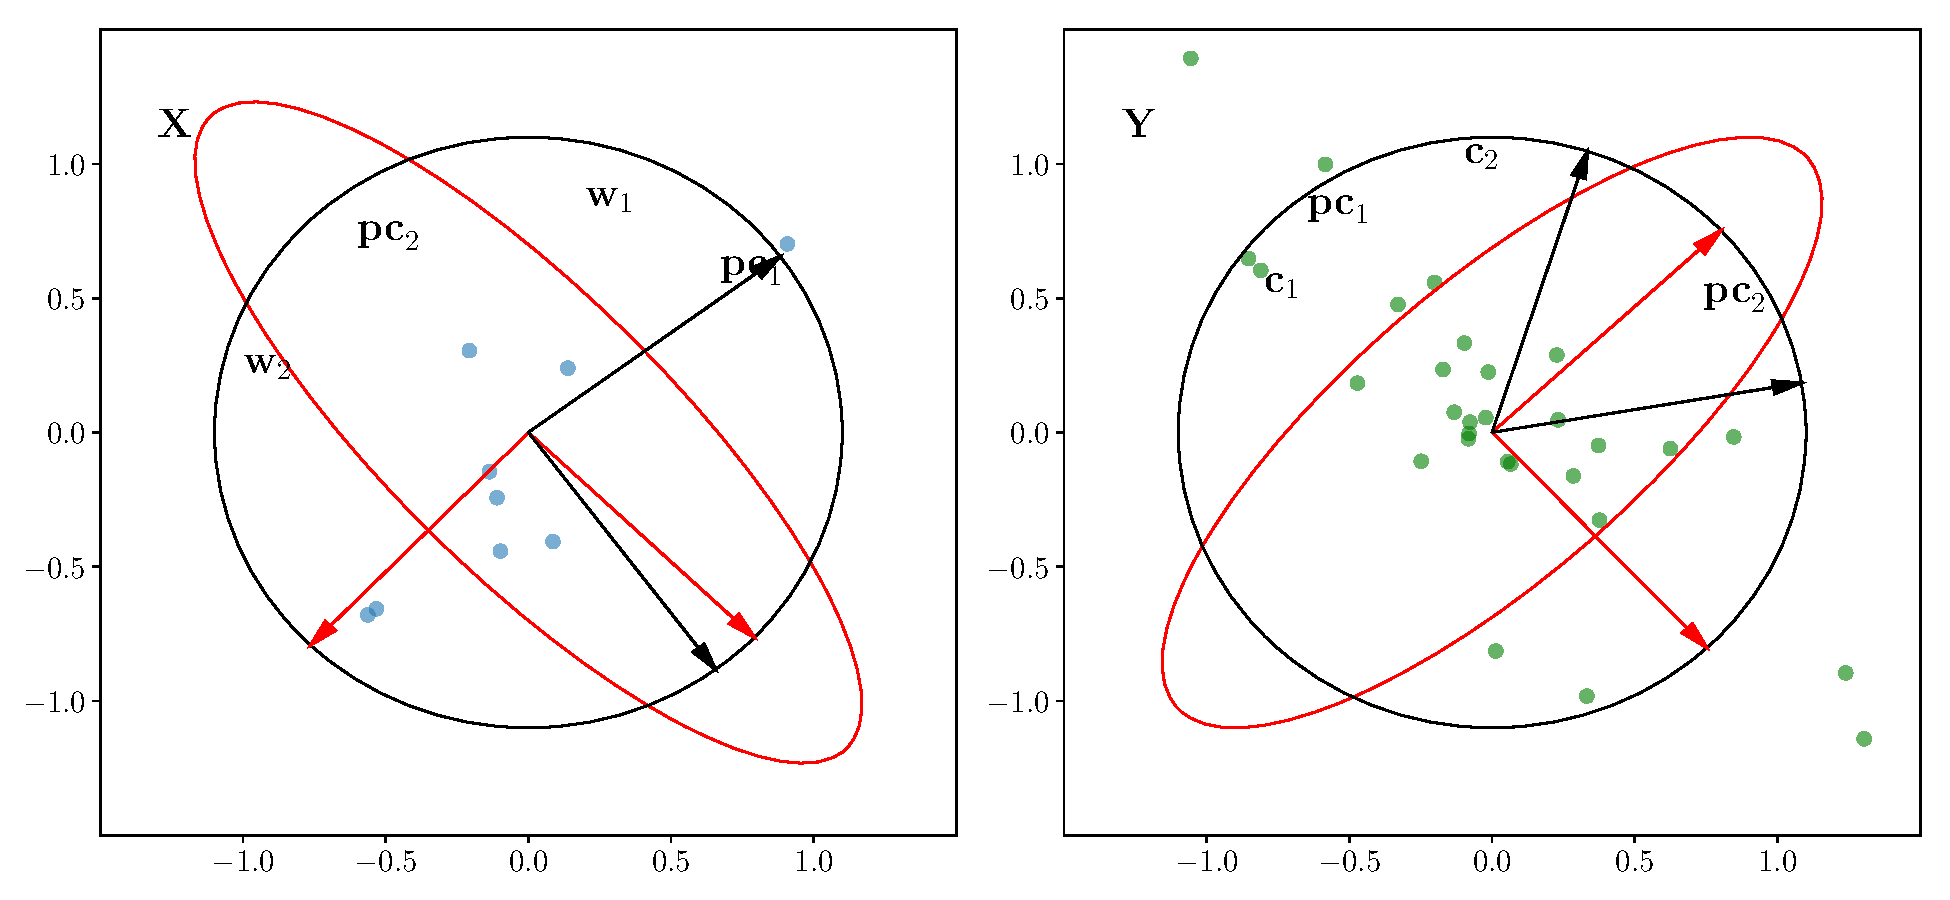
\includegraphics[width=\linewidth]{figs/PLSFigure.pdf}
	\caption{Иллюстрация алгоритма PLS}
	\label{fig::PLSFigure}
\end{figure}

Домножим справа формулу~\eqref{eq::PLS_X} на матрицу $\bW$. Строки матрицы невязок $\bE$ ортогональны столбцам матрицы $\bW$, поэтому 
\[
	\bX \bW = \bT \bP^{\T} \bW.
\] 
Линейное преобразование между объектами в исходном и латентном пространстве имеет вид
\begin{equation}
	\bT = \bX \bW^*,
	\label{eq::W*}
\end{equation}
где $\bW^* = \bW (\bP^{\T} \bW)^{-1}$. Аналогичным образом может быть получена матрица перехода из пространства ответов в латентное пространство $\bC^* = \bC (\bQ^{\T} \bC)^{-1}$.

Матрица параметров модели~\ref{eq::model} находится из уравнений~\eqref{eq::PLS_Y},~\eqref{eq::W*}
\begin{equation*}
    \bY = \bT \bQ^{\T} + \bF = \bX \bW^* \bQ^{\T} + \bF = \bX \bTheta + \bF.
\end{equation*}
Таким образом, 
\begin{equation*}
    \bTheta = \bW (\bP^{\T} \bW)^{-1} \bQ^{\T}.
\end{equation*}

\section{Модификация метода частных наименьших квадратов (cnlPLS)}
Предлагается провести модификацию алгоритма PLS: применить нелинейные параметрические преобразования пространства объектов и ответов для выявления сложных зависимостей.

\begin{align}
\label{eq::PLS_X}
\tilde \bX
= F_x(\bX, \bv_x)
&= \bT\cdot \bP^{\T} + \bE\\
\label{eq::PLS_Y}
\tilde \bY
 = F_y(\bY, \bv_y) 
&= \bT\cdot \bQ^{\T} + \bF,
\end{align}

\subsection{Нелинейные преобразования}

    Рассматриваются нелинейное параметрическое преобразование пространства зависимой переменной $\bY$
    и независимой переменной $\bX$ (примеры преобразований представлены в табл.~\ref{table_functions}). Преобразование и вектор параметров, относящиеся к зависимой переменной и независимой переменной, обозначим соответственно $F_y(\bY, \bv_y)$ и $F_x(\bX, \bv_y)$ и введем переменные для преобразованных пространств
    \begin{equation}
    \label{transf}
        \tilde \bY = F_y (\bY, \bv_y),\quad \tilde \bX = F_x(\bX, \bv_x).
    \end{equation}  

Функции для криволинейных преобразований удовлетворяют следующим условиям:
\begin{itemize}
    \item $F: \mathbb{R} \to \mathbb{R}$,
    \item $F(0) = 0$,
    \item $F$ дифференцируется по параметрам $\bv_y$,
    \item существует $F^{-1}$.
\end{itemize}

\begin{table}[h]
\centering
\begin{tabular}{|l|l|l|}
\hline
\textbf{№} & \textbf{Функция}                                  & \textbf{Параметры} \\ \hline
1          & $F(x) = \sign(x)\exp(a)(\exp(b|x|) - 1)$          & $a, b > 0$         \\ \hline
2          & $F(x) = \sign(x)\exp(a)(\exp(b\ln(1+ \,|x|) - 1)$ & $a, b > 0$         \\ \hline
3          & $F(x) = \sign(x)\exp(a)(\exp(b|x|^{1/2}) - 1)$    & $a, b > 0$         \\ \hline
4          & $F(x) = \sign(x)\exp(a)(\exp(b|x|^{1/3}) - 1)$    & $a, b > 0$         \\ \hline
5          & $F(x) = \sign(x)\exp(a)(\exp(b|x|^{1/4}) - 1)$    & $a, b > 0$         \\ \hline
6          & $F(x) = \sign(x)\exp(a)(\exp(b|x|^{2}) - 1)$      & $a, b > 0$         \\ \hline
\end{tabular}
\caption{Нелинейные преобразования}
\label{table_functions}
\end{table}



Для обучения параметров $\bv_y$ используется градиентный метод. 
Предлагается подход для обновления весов $\bv_y$, основаный на линеаризации функции преобразования. Разложим (\ref{transf}) в ряд Тейлора до второго порядка: 
$$
    \bu \approx \bu_{0} + \frac{\partial \bu}{\partial \bv_y} \Delta \bv_y.
$$
    
Для вычисления $\Delta \bv_y$ предложены следующие шаги. Рассматривается разница $\bu - \bu_{0} = \frac {\partial \bu}{\partial \bv_y} \Delta \bv_y$. Определется рассогласование
$$
    \bu - \bu_{0} \approx \frac {\partial \bu}{\partial \bv_y} \Delta \bv_y = \bJ_u \Delta \bv_y,
$$
где матрица $\bJ_u$ состоит из частных производных $\left\{\frac {\partial \bu}{\partial \bv_y} \right\}$, вычисленных при известном значении переменной $\bu$: 
\[
    \bJ_u = \frac {\partial \bu}{\partial \bv_y} 
    = \frac {\partial }{\partial \bv_y} (\tilde \bY \bc)
    = \frac1{(\bt^{\T}\bt)} \frac {\partial }{\partial \bv_y} \left(\tilde \bY \tilde \bY^{\T}\bt \right) 
    = \frac{1}{(\bt^{\T}\bt)} \left( \frac {\partial \tilde \bY }{\partial \bv_y}  \cdot \tilde \bY^{\T}  + \tilde \bY \cdot \frac {\partial \tilde \bY^{\T}  }{\partial \bv_y}  \right) \bt.
\]

Правило обновления для вектора $\Delta \bv$ является решением задачи регрессии рассогласования
\begin{equation}
\label{delta_v}
\Delta \bv_y  = (\bJ_u^{\T} \bJ_u)^{-1} \bJ_u^{\T} (\bu - \bu_0).
\end{equation}


Аналогично преобразованию зависимой переменной сводим задачу обновления вектора параметров $\bv_x$ к задаче линейной регрессии:

\begin{align*}
    \bt - \bt_0 \approx \frac {\partial \bt}{\partial \bv_x} \Delta \bv_x = \bJ_t \Delta \bv_x \\
    \Delta \bv_x  = (\bJ_t^{\T} \bJ_t)^{-1} \bJ_t^{\T} (\bt - \bt_0).
\end{align*}

\subsection{Алгоритм cnlPLSR}
В данном разделе представлен модифицированный метод PLSR, содержащий шаги преобразования целевой переменной. Аналогично методу PLSR (алгоритм~\ref{PLSR_pseudo}), алгоритм \ref{cnlPLSR_pseudo} начинается с инициализации вектора $\bu$, а обновления весов преобразования считается с помощью рассогласования $\be$ для вектора $\bu$, вычисленного в цикле и на предыдущей итерации.
\vspace{-0.5cm}

\begin{center}
\begin{algorithm}[h]
\caption{Алгоритм cnlPLSR с преобразованием пространства объектов 2}
    \label{cnlPLSR_pseudo_x}
\begin{algorithmic}[1]
\REQUIRE $\bX, \bY, l$;
\ENSURE $\bT, \bP, \bQ, \bv_x, \bv_y$;
\STATE инициализировать $\bv_x$ и $\bv_y$
\STATE нормировать матрицы $\bX, \bY$
\STATE $\bX_1 = \bX; \bY_1 = \bY$
\FOR{$k=1,\dots, l$}
\STATE инициализировать $\bt_0$ (первый столбец матрицы $\bX$)
\STATE инициализировать $\bu_0$ (первый столбец матрицы $\bY$)
  \REPEAT
  \vspace{0.1cm}
    \STATE $\tilde \bX_k := F_x(\bX_k, \bv_x); \quad \tilde \bY_k = F_y(\bY_k, \bv_y)$
    \vspace{0.1cm}
    \STATE $\bw_k := \tilde \bX_k^{\T} \bu_{k-1} / (\bu_{k-1}^{\T} \bu_{k-1}); \quad \bw_k: = \frac{\bw_k}{\|\bw_k \|}$
    \STATE $\bt_k := \tilde \bX_k \bw_k$
    \vspace{0.1cm}
    \STATE $\Delta \bv_x = (\bJ_t^{\T} \bJ_t)^{-1} \bJ_t^{\T} (\bt_k - \bt_{k-1})$, где $\bJ_t := \frac{\partial \bt_k}{\partial \bv_x}$
    \vspace{0.1cm}
    \STATE $\bv_x := \bv_x + \Delta \bv_x$
    \vspace{0.1cm}
    \STATE $\bc_k := \tilde \bY_k^{\T} \bt_k / (\bt_k^{\T} \bt_k); \quad \bc_k: = \frac{\bc_k}{\| \bc_k \|}$ 
    \STATE $\bu_k := \tilde \bY_k \bc_k$
    \vspace{0.1cm}
    \STATE $\Delta \bv_y = (\bJ_u^{\T} \bJ_u)^{-1} \bJ_u^{\T} (\bu_k - \bu_{k-1})$, где $\bJ_u := \frac{\partial \bu_k}{\partial \bv_y}$
    \vspace{0.1cm}
    \STATE $\bv_y := \bv_y + \Delta \bv_y$
  \UNTIL{$\bt_k$ не стабилизируется}
   \vspace{0.1cm}
 \STATE $\bp_k := \tilde \bX_k^{\T}\bt_k/(\bt_k^{\T}\bt_k),\ \bq_k := \tilde \bY_k^{\T}\bt_k/(\bt_k^{\T}\bt_k)$
 \vspace{0.1cm}
 \STATE $\tilde \bX_k := \tilde  \bX_k - \bt_k \bp_k^{\T}$
 \vspace{0.1cm}
 \STATE $\tilde \bY_k := \tilde  \bY_k - \bt_k\bq_k^{\T}$ 
 \vspace{0.1cm}
  \STATE $\bX_k = F_x^{-1}(\tilde \bX_k, \bv_x)$; $\bY_k = F_y^{-1}(\tilde \bY_k, \bv_y)$
\ENDFOR
\end{algorithmic}
\end{algorithm}
\end{center}

%%%%%%%%%%%%%%%%%%%%%%%%%%%%%%%%%%%%%%%%%%%%%%%%%%%%%%%%%%%%%%%%%%%%%%%%%%%%%%
\newpage
\section{Вычислительный эксперимент}
%%%%%%%%%%%%%%%%%%%%%%%%%%%%%%%%%%%%%%%%%%%%%%%%%%%%%%%%%%%%%%%%%%%%%%%%%%%%%%

В случае данных электроэнергии $i$-ая строка  матрицы $\bX$~--– локальная история сигнала ($n$ значений сигнала, начиная с момента $i$), а $i$-ая строка матрицы $\bY$~--– локальный прогноз, то есть $r$ значений сигнала, начиная с момента $n+1$. В случае данных ECoG матрица $\bX$ состоит из пространственно-временного спектрального представления временных рядов напряжения, а матрица $\bY$ содержит информацию о положении руки. Процесс генерации матрицы $\bX$ из значений напряжения описан в (ссылка на Мотренко). 

В рамках вычислительного эксперимента строится прогноз временных рядов. В ходе эксперимента сравниваются методы PLSR, нелинейных автоэнкодеров и cnlPLS. Сравнение проводится на реальных данных объемов потребления электроэнергии в Польше. 

Вычислительный эксперимент, продемонстрированный в этом разделе, основан на данных электроэнергии. Данные состоят из временного ряда польских электрических нагрузок и временных рядов погоды в Варшаве (долгота: 21,25, широта: 52,30, высота над уровнем моря: 94). Временные ряды энергии состоят из почасовых записей (всего 52512 наблюдений), а погодные измерения проводились раз в день и содержат 2188 наблюдений. Многомасштабные временные ряды соответствуют периоду 1999-2004 годов. Результаты, полученные с этим набором данных, являются иллюстрацией предлагаемых методов, поскольку данные содержат многомасштабне временные ряды, имеющие различный характер.

Примеры работы алгоритма приведены на рис.~\ref{fig:forecast}. Метод успешно делает краткосрочный прогноз (до 10 дней). С увеличением горизонта прогнозирования предсказание смещается. 


% Require \usepackage{subfig}

% \begin{figure}[H]
%     \centering
%     \begin{subfigure}[b]{0.3\textwidth}
%         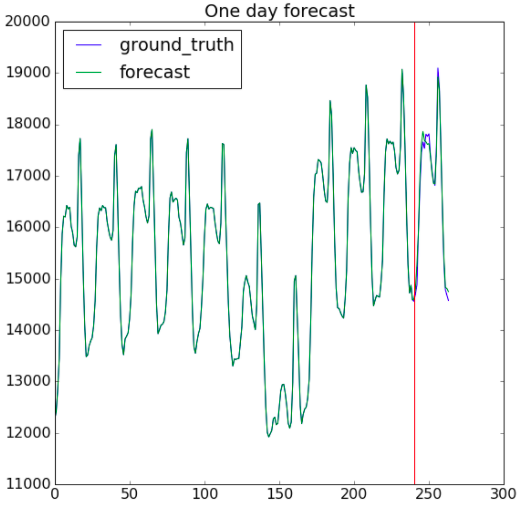
\includegraphics[width=\textwidth]{oneday.png}
%     \end{subfigure}
%     \begin{subfigure}[b]{0.3\textwidth}
%         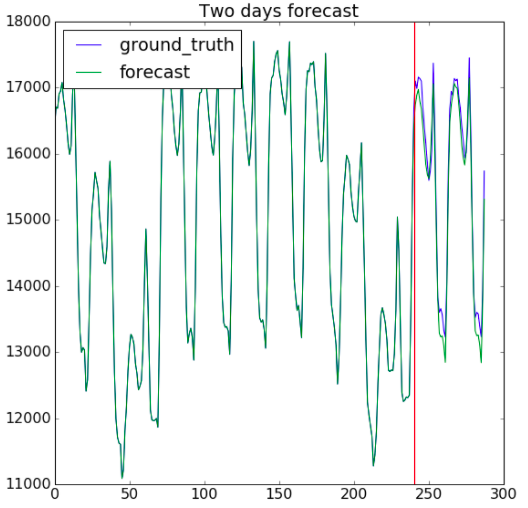
\includegraphics[width=\textwidth]{twodays.png}
%     \end{subfigure}
%     \begin{subfigure}[b]{0.3\textwidth}
%         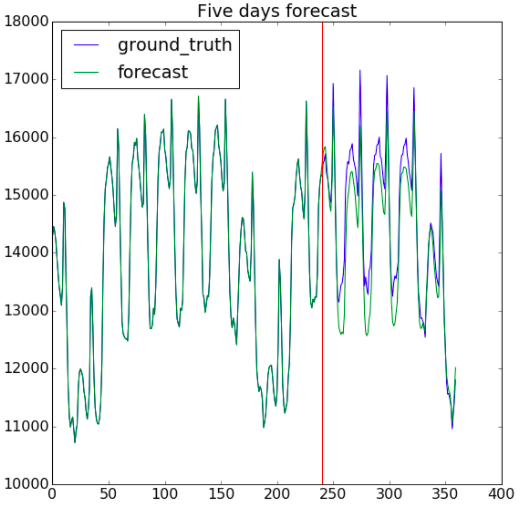
\includegraphics[width=\textwidth]{fivedays.png}
%     \end{subfigure}
%     \begin{subfigure}[b]{0.3\textwidth}
%         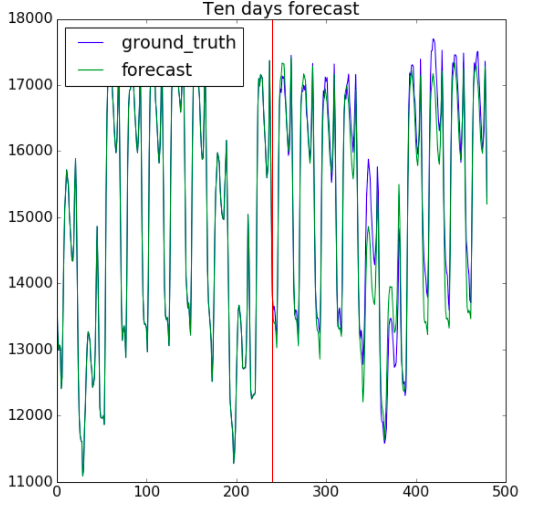
\includegraphics[width=\textwidth]{tendays.png}
%     \end{subfigure}
%     \begin{subfigure}[b]{0.3\textwidth}
%         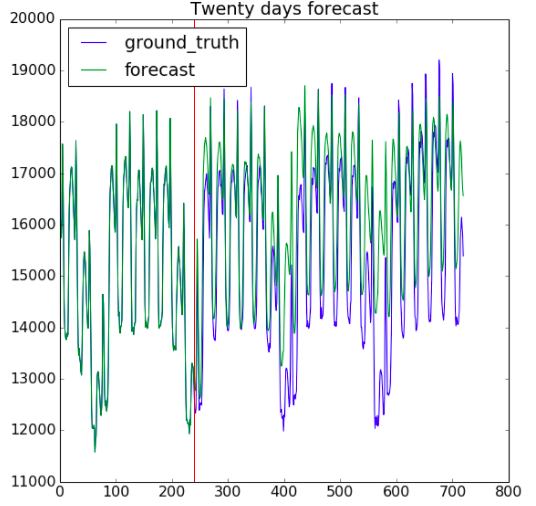
\includegraphics[width=\textwidth]{twentydays.png}
%     \end{subfigure}
%     \begin{subfigure}[b]{0.3\textwidth}
%         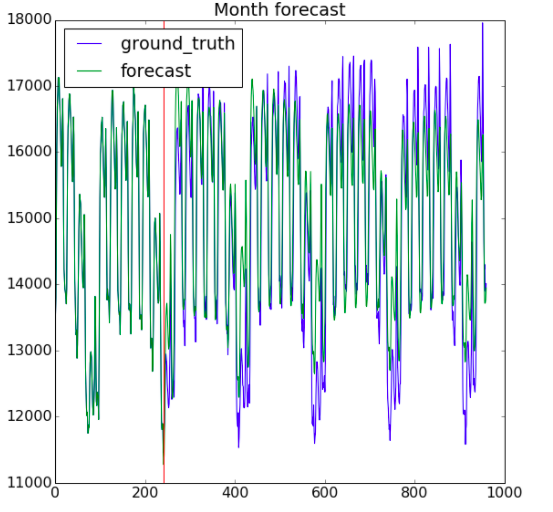
\includegraphics[width=\textwidth]{month.png}
%     \end{subfigure}
%     \caption{Прогнозирование базового алгоритма на 1, 2, 5, 10, 20, 30 дней}
%     \label{fig:forecast}
% \end{figure}

Результаты вычислительного эксперимента для предложенного модифицированного алгоритма cnlPLS представлены на рис.~\ref{fig:animals}. На графиках изображены сглаженные зависимости ошибки MSE от числа компонент в алгоритме для разных функций. Из графиков видно, что для функций $(a)-(e)$ ошибка при увеличении числа компонент падает, затем колеблется, слабо меняясь. Ошибка алгоритма с функцией $(f)$ увеличивается при увеличении числа компонент. Это означает, что преобразование, выполненное в пространстве целевой переменной с помощью функции $(f)$, плохо описывает зависимость. Меньшую ошибку имеют функции, растущие медленнее, а именно $(d)$ и $(e)$. 



% Require \usepackage{subfig}

% \begin{figure}
%     \centering
%     \begin{subfigure}[b]{0.4\textwidth}
%         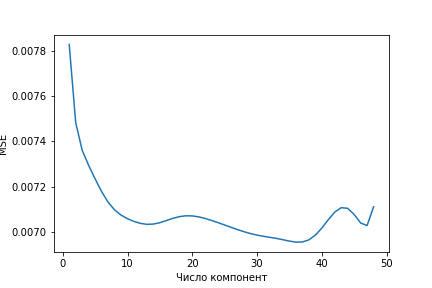
\includegraphics[width=\textwidth]{exp_abs_x.png}
%         \caption{$g(x) = \sign(x) e^a(\exp(b|x|) - 1)$}
%         \label{fig:exp_abs_x}
%     \end{subfigure}
%     ~ %add desired spacing between images, e. g. ~, \quad, \qquad, \hfill etc. 
%       %(or a blank line to force the subfigure onto a new line)
%     \begin{subfigure}[b]{0.4\textwidth}
%         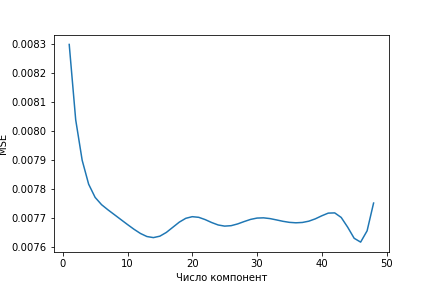
\includegraphics[width=\textwidth]{exp_log_x.png}
%         \caption{$g(x) = \sign(x)e^a(\exp(b\ln(1+ \,|x|) - 1)$}
%         \label{fig:exp_log_x}
%     \end{subfigure}
%     ~ %add desired spacing between images, e. g. ~, \quad, \qquad, \hfill etc. 
%     %(or a blank line to force the subfigure onto a new line)
%     \begin{subfigure}[b]{0.4\textwidth}
%         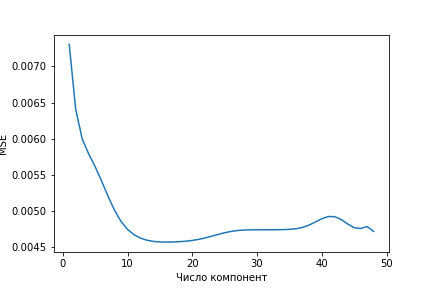
\includegraphics[width=\textwidth]{exp_x_1_2.png}
%         \caption{$g(x) = \sign(x)e^a(\exp(b|x|^{1/2}) - 1)$}
%         \label{fig:exp_x_1_2}
%     \end{subfigure}
%     \begin{subfigure}[b]{0.4\textwidth}
%         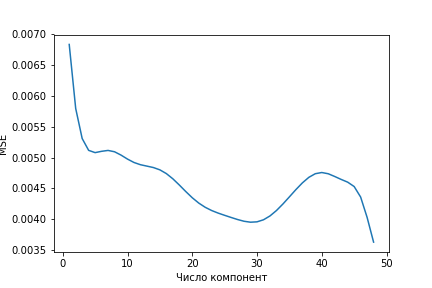
\includegraphics[width=\textwidth]{exp_x_1_3.png}
%         \caption{$g(x) = \sign(x)e^a(\exp(b|x|^{1/3}) - 1)$ }
%         \label{fig:exp_x_1_3}
%     \end{subfigure}
%     ~ %add desired spacing between images, e. g. ~, \quad, \qquad, \hfill etc. 
%       %(or a blank line to force the subfigure onto a new line)
%     \begin{subfigure}[b]{0.4\textwidth}
%         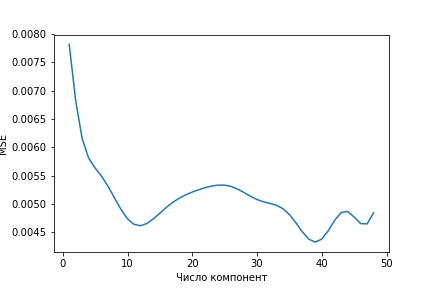
\includegraphics[width=\textwidth]{exp_x_1_4.png}
%         \caption{$g(x) = \sign(x)e^a(\exp(b|x|^{1/4}) - 1)$}
%         \label{fig:exp_x_1_4}
%     \end{subfigure}
%     ~ %add desired spacing between images, e. g. ~, \quad, \qquad, \hfill etc. 
%     %(or a blank line to force the subfigure onto a new line)
%     \begin{subfigure}[b]{0.4\textwidth}
%         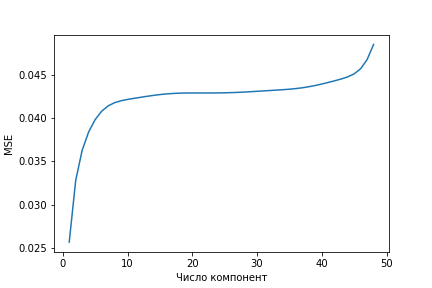
\includegraphics[width=\textwidth]{exp_x_2.png}
%         \caption{$g(x) = \sign(x)e^a(\exp(b|x|^{2}) - 1)$}
%         \label{fig:exp_x_2}
%     \end{subfigure}
%     \caption{Зависимость ошибки от числа компонент в алгоритме cnlPLS для разных функций}\label{fig:animals}
% \end{figure}

В табл.~\ref{results} продемонстрировано увеличение точности прогнозивания при использовании криволинейного преобразования в пространстве зависимой переменной, но увеличение точности в пределах погрешности алгоритма (0.0005-0.0010). Функции с быстрым ростом не позволяют описать зависимость.
\begin{table}[]
\centering
\begin{tabular}{|l|l|l|l|l|}
\hline
\textbf{Алгоритм}                                                                                  & \textbf{N=3}     & \textbf{N=5}     & \textbf{N=10}    & \textbf{N=20}    \\ \hline
PLS                                                                                                & 0,00404          & 0,00337          & \textbf{0,00151} & 0,00135          \\ \hline
\begin{tabular}[c]{@{}l@{}}cnlPLS\\ $g(x) = \sign(x)\exp(a)(\exp(b|x|) - 1)$\end{tabular}          & 0.00529          & 0.00514          & 0.00536          & 0.00506          \\ \hline
\begin{tabular}[c]{@{}l@{}}cnlPLS\\ $g(x) = \sign(x)\exp(a)(\exp(b\ln(1+ \,|x|) - 1)$\end{tabular} & 0.00362          & 0.00386          & 0.00326          & 0.00317          \\ \hline
\begin{tabular}[c]{@{}l@{}}cnlPLS\\ $g(x) = \sign(x)\exp(a)(\exp(b|x|^{1/2}) - 1)$\end{tabular}    & 0.00272          & 0.00236          & 0.00287          & \textbf{0.00128} \\ \hline
\begin{tabular}[c]{@{}l@{}}cnlPLS\\ $g(x) = \sign(x)\exp(a)(\exp(b|x|^{1/3}) - 1)$\end{tabular}    & \textbf{0.00241} & \textbf{0.00233} & 0.00221          & 0.00173          \\ \hline
\begin{tabular}[c]{@{}l@{}}cnlPLS\\ $g(x) = \sign(x)\exp(a)(\exp(b|x|^{1/4}) - 1)$\end{tabular}    & 0.00796          & 0.00768          & 0.00737          & 0.00803          \\ \hline
\begin{tabular}[c]{@{}l@{}}cnlPLS\\ $g(x) = \sign(x)\exp(a)(\exp(b|x|^{2}) - 1)$\end{tabular}      & 0.00816          & 0.00798          & 0.00796          & 0.00775          \\ \hline
\end{tabular}
\caption{Значения ошибки MSE для разных чисел компонент и разных функций}
\label{results}
\end{table}

%%%%%%%%%%%%%%%%%%%%%%%%%%%%%%%%%%%%%%%%%%%%%%%%%%%%%%%%%%%%%%%%%%%%%%%%%%%%%%
\section{Заключение}
В данной работе предложен новый подход к обнаружению зависимостей в пространстве зависимой переменной задачи прогнозирования временных рядов. Сравнивались результаты прогнозирования временных рядов, полученных с помощью метода частных наименьших квадратов и предложенной модификации. Проведен вычислительный эксперимент на реальных данных потребления электроэнергии в Варшаве. Построенная прогностическая модель показала высокое качество предсказания электрической нагрузки. 
%%%%%%%%%%%%%%%%%%%%%%%%%%%%%%%%%%%%%%%%%%%%%%%%%%%%%%%%%%%%%%%%%%%%%%%%%%%%%%
%\section*{СПИСОК ЛИТЕРАТУРЫ}

\newpage
\nocite{*}

\bibliographystyle{unsrt}
\begin{thebibliography}{10}
\def\selectlanguageifdefined#1{
\expandafter\ifx\csname date#1\endcsname\relax
\else\selectlanguage{#1}\fi}

\bibitem{thrun2012}
\BibAuthor{Thrun, Sebastian and Pratt, Lorien}
{Learning to learn}~//
Springer Science \& Business Media, 2012.

\bibitem{Chong2005} %1
%\selectlanguageifdefined{english}
\BibAuthor{Chong, Il Gyo and Jun, Chi Hyuck}
{Performance of some variable selection methods when multicollinearity is present}~//
Chemometrics and Intelligent Laboratory Systems, 2005.
Vol.~78.
No.~1.
P.~103--112.

\bibitem{Xuefeng2010} %1
%\selectlanguageifdefined{english}
\BibAuthor{Xuefeng, Yan}
{Hybrid artificial neural network based on BP-PLSR and its application in development of soft sensors}~//
Chemometrics and Intelligent Laboratory Systems, 2010.
Vol.~103.
No.~2.
P.~152--159.

\bibitem{Mcavovt1992} %1
%\selectlanguageifdefined{english}
\BibAuthor{Mcavovt, J. and Process, Chemical}
{Title }~//
Journal name, 2005.
Vol.~16.
No.~4.
P.~379--391.

\bibitem{Yan2003} %1
%\selectlanguageifdefined{english}
\BibAuthor{Yan, Xuefeng F. and Chen, Dezhao Z. and Hu, Shangxu X.}
{Chaos-genetic algorithms for optimizing the operating conditions based on RBF-PLS model}~//
Computers and Chemical Engineering, 2003.
Vol.~27.
No.~10.
P.~1393--1404.

\bibitem{Frank1990} %1
%\selectlanguageifdefined{english}
\BibAuthor{Frank, Ildiko E.}
{A nonlinear PLS model}~//
Chemometrics and Intelligent Laboratory Systems, 1990.
Vol.~8.
No.~2.
P.~109--119.

\bibitem{Zhou2007} %1
%\selectlanguageifdefined{english}
\BibAuthor{Zhou, Yan Ping and Jiang, Jian Hui and Lin, Wei Qi and Xu, Lu and Wu, Hai Long and Shen, Guo Li and Yu, Ru Qin}
{Artificial neural network-based transformation for nonlinear partial least-square regression with application to QSAR studies}~//
Talanta, 2007.
Vol.~71.
No.~2.
P.~848--853.


\bibitem{Geladi1988} %1
%\selectlanguageifdefined{english}
\BibAuthor{Chong, Il Gyo and Jun, Chi Hyuck}
{Notes on the history and nature of partial least squares (PLS) modelling}~//
Journal of Chemometrics, 1988.
Vol.~2.
No.~January.
P.~231--246.


\bibitem{Hoskuldsson1988} %1
%\selectlanguageifdefined{english}
\BibAuthor{H{\"{o}}skuldsson, Agnar}
{PLS regression}~//
Chemometrics and Intelligent Laboratory Systems, 1987.
Vol.~2.
No.~August.
P.~581--591.


\bibitem{Bulut2014} %1
%\selectlanguageifdefined{english}
\BibAuthor{Bulut, Elif and Egrioglu, Erol}
{A New Partial Least Square Method Based on Elman Neural Network}~//
Chemometrics and Intelligent Laboratory Systems, 2005.
Vol.~4.
No.~4.
P.~154--158.


\bibitem{Ng2013} %1
%\selectlanguageifdefined{english}
\BibAuthor{Ng, Kee Siong}
{A Simple Explanation of Partial Least Squares}~//
Journal title, 2013.
Vol.~volume.
No.~number.
P.~1--10.


\bibitem{Rosipal2011} %1
%\selectlanguageifdefined{english}
\BibAuthor{Rosipal, Roman}
{Nonlinear partial least squares: An overview}~//
Chemoinformatics and Advanced Machine Learning Perspectives: Complex Computational Methods and Collaborative Techniques, 2011.
Vol.~number.
No.~number.
P.~169--189.


\bibitem{Wold1989} %1
%\selectlanguageifdefined{english}
\BibAuthor{Wold, Svante and Kettaneh-Wold, Nouna and Skagerberg, Bert}
{Nonlinear PLS modeling}~//
Chemometrics and Intelligent Laboratory Systems, 1989.
Vol.~7.
No.~1-2.
P.~53--65.

\bibitem{Rosipal2006} %1
%\selectlanguageifdefined{english}
\BibAuthor{Rosipal, Roman and Kramer, Nicole}
{Overview and Recent Advances in Partial Least Squares}~//
????? C. Saunders et al. (Eds.): SLSFS 2005, LNCS 3940, 2006.
Vol.~?.
No.~?.
P.~34--51.

\bibitem{Lu2004} %1
%\selectlanguageifdefined{english}
\BibAuthor{Lu, Wen-Cong and Chen, Nian-Yi and Li, Guo-Zheng and Yang, Jie}
{Multitask Learning Using Partial Least Squares Method}~//
Proceedings of the Seventh International Conference on Information Fusion; International Society of Information Fusion, 2004.
Vol.~1.
P.~79--84.

\bibitem{Varnek2012} %1
%\selectlanguageifdefined{english}
\BibAuthor{Varnek, Alexandre and Baskin, Igor}
{Machine learning methods for property prediction in chemoinformatics: Quo Vadis?}~//
Journal of Chemical Information and Modeling, 2012.
Vol.~52.
No.~6.
P.~1413--1437.

\bibitem{Lehky2014} %1
%\selectlanguageifdefined{english}
\BibAuthor{Lehky, Sidney R. and Kiani, Roozbeh and Esteky, Hossein and Tanaka, Keiji}
{Dimensionality of object representations in monkey inferotemporal cortex}~//
Neural computation, 2014.
Vol.~1872.
No.~10.
P.~1840--1872.

\bibitem{Abdi2003} %1
%\selectlanguageifdefined{english}
\BibAuthor{Abdi, Herv{\'{e}}}
{Partial Least Squares (PLS) Regression}~//
Encyclopedia for research methods for the social sciences, 2003.
P.~792--795.

\bibitem{Caruana2003} %1
%\selectlanguageifdefined{english}
\BibAuthor{Caruana, Rich and de Sa, Virginia R.}
{Benefitting from the Variables that Variable Selection Discards}~//
Journal of Machine Learning Research, 2003.
Vol.~3.
No.~7-8.
P.~1245--1264.

\bibitem{Mises1929} %1
%\selectlanguageifdefined{english}
\BibAuthor{Mises R. V., Pollaczek‐Geiringer H. }
{Praktische Verfahren der Gleichungsauflösung}~//
ZAMM‐Journal of Applied Mathematics and Mechanics/Zeitschrift für Angewandte Mathematik und Mechanik, 1929.
Vol.~9.
No.~1.
P.~58--77.

\bibitem{Li2016} %1
%\selectlanguageifdefined{english}
\BibAuthor{Li J. et al.}
{Feature selection: A data perspective}~//
arXiv preprint arXiv:1601.07996, 2016.


\end{thebibliography}


\end{document}